\documentclass[11pt,a4paper]{article}

\usepackage[margin=1.05in]{geometry}
\usepackage{amsmath,amssymb,amsthm}
\usepackage{stmaryrd}
\usepackage{booktabs}
\usepackage{microtype}
\usepackage{xcolor}
\usepackage{listings}
\usepackage{tikz}
\usetikzlibrary{arrows.meta,positioning,fit,backgrounds}
\usepackage[htt]{hyphenat}   % allow long \texttt identifiers to break
\usepackage[hidelinks]{hyperref}

% ---------------------------------------------------------------- notation
\newcommand{\sem}[1]{\llbracket #1 \rrbracket}
\newcommand{\seme}[2]{\llbracket #1 \rrbracket_{#2}}
\newcommand{\Bool}{\mathbb{B}}
\newcommand{\Real}{\mathbb{R}}
\newcommand{\Rat}{\mathbb{Q}}
\newcommand{\VC}{\mathrm{VCGen}}
\newcommand{\VCd}{\mathrm{VCGen}_{\div}}
\newcommand{\Conserves}{\mathrm{Conserves}}
\newcommand{\DivSafe}{\mathrm{DivisionSafe}}
\newcommand{\unsat}{\mathsf{unsat}}
\newcommand{\sat}{\mathsf{sat}}
\newcommand{\unknown}{\mathsf{unknown}}
\newcommand{\code}[1]{\texttt{#1}}

\theoremstyle{definition}
\newtheorem{definition}{Definition}[section]
\newtheorem{example}[definition]{Example}
\theoremstyle{plain}
\newtheorem{theorem}[definition]{Theorem}
\newtheorem{lemma}[definition]{Lemma}
\theoremstyle{remark}
\newtheorem*{intuition}{Intuition}
\newtheorem*{warning}{Caution}

\lstdefinestyle{plain}{
  basicstyle=\ttfamily\small,
  breaklines=true,
  frame=single,
  rulecolor=\color{gray!45},
  framesep=5pt,
  showstringspaces=false,
  columns=fullflexible,
  keepspaces=true,
}
\lstset{style=plain}

% Long \code{...} identifiers must be breakable or they overflow the measure.
\emergencystretch=2.5em
\hyphenpenalty=1000

\title{\textbf{Proving Properties of Compiled Daml Packages}\\[
  0.35em]\large A guided introduction to the verification pipeline}
\author{Daml Access Graph}
\date{}

\begin{document}
\maketitle

\begin{abstract}
\noindent
This document explains how the verification pipeline in this repository proves
properties of a compiled Daml package, and, just as importantly, what its
results do not mean. It is written to be read start to finish by someone who
knows Daml but not formal verification. Section~\ref{sec:worked} carries a
single example the whole way through, from a Daml choice to a solver verdict,
before any general theory appears. The formal companion to this document is
\code{formal/SPECIFICATION.md} (definitions and theorems, stated tersely) and
\code{formal/Correspondence.md} (the trust audit).
\end{abstract}

\tableofcontents
\bigskip

% =============================================================== 1
\section{The problem}

Suppose we want to know that a token package never loses value: whenever a
choice archives a contract and creates replacements, the amounts add up. A test
suite can sample this. It cannot establish it, because a choice takes arguments
from an infinite domain and a test tries finitely many.

The alternative is to prove it. That raises a question which is easy to state
and easy to get wrong.

\subsection{The correspondence gap}

A proof is always a proof \emph{about some model}. If we write a symbolic model
of a contract by hand and verify the model, we have established
\[
  M \models \varphi
\]
for our hand-built $M$. Whether $M$ faithfully describes the contract $C$ that
is actually deployed is a separate claim,
\[
  \sem{C} = M,
\]
and in most developments that claim is an unproven comment. It is also where
the interesting bugs live: a model drifts from its implementation silently, and
a verified model of the wrong thing is worse than no model at all, because it
carries the authority of a proof.

\begin{intuition}
Verifying a hand-written model answers ``is my description of the contract
correct?'' We want an answer to ``is the contract correct?'' The two coincide
only if the description matches, and that match is exactly what a hand-written
model leaves unchecked.
\end{intuition}

This pipeline attacks the gap directly by deriving the model from the compiled
artifact. Nothing is transcribed by hand. The DAR that would be deployed is the
input, and the transition system is extracted from it. For the fragment the
translator handles, the correspondence holds by construction; where the
translator cannot proceed, it says so in the output rather than guessing.

\subsection{The pipeline}

\begin{center}
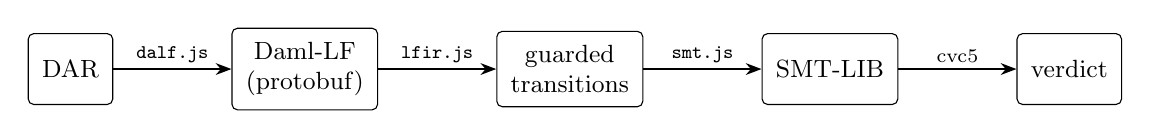
\begin{tikzpicture}[
  node distance=15mm,
  box/.style={draw,rounded corners=2pt,align=center,inner sep=5pt,
              font=\small,minimum height=9mm},
  ar/.style={-{Stealth[length=2mm]},semithick},
  lbl/.style={above,font=\scriptsize,inner sep=2pt},
]
\node[box] (dar) {DAR};
\node[box,right=of dar] (lf) {Daml-LF\\(protobuf)};
\node[box,right=of lf] (ir) {guarded\\transitions};
\node[box,right=of ir] (smt) {SMT-LIB};
\node[box,right=of smt] (v) {verdict};

\draw[ar] (dar) -- node[lbl] {\code{dalf.js}} (lf);
\draw[ar] (lf)  -- node[lbl] {\code{lfir.js}} (ir);
\draw[ar] (ir)  -- node[lbl] {\code{smt.js}} (smt);
\draw[ar] (smt) -- node[lbl] {cvc5} (v);
\end{tikzpicture}
\end{center}

\noindent
The claim proved in Lean, for the fragment of Section~\ref{sec:gap}, is
\begin{equation}
  \label{eq:central}
  \boxed{\;\models \VC(P, \varphi) \;\Longrightarrow\; P \models \varphi\;}
\end{equation}
read as: if the generated verification condition is valid, the package really
does satisfy the property. The solver establishes the left-hand side. The
theorem is what licenses the step to the right-hand side.

% =============================================================== 2
\section{A complete worked example}
\label{sec:worked}

Before any general definitions, here is the entire pipeline on one choice. The
example is a \emph{split}: a contract holding an amount is archived, and two
contracts are created holding $x$ and the remainder.

\subsection{The source}

\begin{lstlisting}
choice Split : (ContractId Piece, ContractId Piece)
  with x : Decimal
  controller owner
  do
    a <- create Piece with amount = x
    b <- create Piece with amount = this.amount - x
    pure (a, b)
\end{lstlisting}

\noindent
The property we want is that the split conserves value: the two pieces together
hold exactly what the archived contract held.

\subsection{The extracted transition}

The translator reduces the choice to the data the property needs: the guards
that must hold, the amounts assigned by each \code{create}, and the amount of
the contract being archived. Variables are named by the projection path that
produced them, so \code{arg.x} is the choice argument and \code{this.amount} is
a field of the exercised contract.
\[
  \tau \;=\; \bigl\langle\;
    \underbrace{[\,]}_{\text{guards}},\;\;
    \underbrace{[\;\code{arg.x},\;\; \code{this.amount} - \code{arg.x}\;]}_{\text{created amounts}},\;\;
    \underbrace{\code{this.amount}}_{\text{archived}}
  \;\bigr\rangle
\]
This is \code{splitTransition} in \code{formal/Formal/Ledger.lean}, where it
serves the same illustrative purpose.

\subsection{The property}

Conservation says: in every environment where the guards hold, the created
amounts sum to the archived amount. There are no guards here, so the condition
is unconditional:
\[
  \forall \rho.\quad
  \seme{\code{arg.x}}{\rho} + \bigl(\seme{\code{this.amount}}{\rho} - \seme{\code{arg.x}}{\rho}\bigr)
  \;=\; \seme{\code{this.amount}}{\rho}
\]
Here $\rho$ is an \emph{environment}: an assignment of a rational number to
every variable name. Quantifying over all of them is what makes the result a
proof rather than a sample.

\subsection{The verification condition}

We do not ask the solver ``is this true?'' Solvers answer satisfiability
questions, so we ask the dual: \emph{is there any environment making the
property false?} We assert the guards, assert the negation of the goal, and ask
whether the set has a model.

\begin{lstlisting}
(declare-fun |arg.x| () Real)
(declare-fun |this.amount| () Real)
(assert (not (= (+ |arg.x| (- |this.amount| |arg.x|)) |this.amount|)))
(check-sat)
\end{lstlisting}

\noindent
cvc5 answers $\unsat$: no such environment exists. No counterexample exists,
so the property holds in every environment, and the verdict is \code{PROVED}.

\begin{intuition}
$\unsat$ is the good answer. It means the search for a counterexample was
exhaustive and came back empty. A $\sat$ answer hands back a concrete
environment, which is why counterexamples can be printed but proofs cannot.
\end{intuition}

\subsection{Where the theorem enters}

The solver proved a fact about a \emph{formula}. We want a fact about a
\emph{choice}. Three steps separate them, and each is discharged differently:

\begin{center}
\begin{tabular}{@{}lll@{}}
\toprule
Step & Justified by & Status \\
\midrule
choice $\to$ transition & \code{lfir.js} & tested; proved on a fragment \\
transition $\to$ formula & $\VC$, Theorem~\ref{thm:sound} & machine-checked \\
formula $\to$ $\unsat$ & cvc5 & trusted \\
\bottomrule
\end{tabular}
\end{center}

\noindent
The middle row is the one this development contributes. The rest of the
document makes it precise, then returns to the outer two rows, which are where
the residual risk lives.

% =============================================================== 3
\section{The intermediate representation}

\subsection{Syntax}

Terms are indexed by a sort, either real or boolean.

\begin{definition}[Sorts and terms]
$s ::= \Real \mid \Bool$, and terms $t : \mathrm{Term}\,s$ are generated by
\[
\begin{aligned}
t^{\Real} \;::=\;& q \;\mid\; x^{\Real}
  \;\mid\; t_1 + t_2 \;\mid\; t_1 - t_2 \;\mid\; t_1 \cdot t_2
  \;\mid\; t_1 / t_2 \;\mid\; t_1 \mathbin{\mathrm{div}} t_2 \;\mid\; t_1 \bmod t_2 \\
t^{\Bool} \;::=\;& b \;\mid\; x^{\Bool}
  \;\mid\; t_1 < t_2 \;\mid\; t_1 \le t_2 \;\mid\; t_1 > t_2 \;\mid\; t_1 \ge t_2 \\
  &\mid\; t_1 =_{\Real} t_2 \;\mid\; t_1 =_{\Bool} t_2
  \;\mid\; \neg t \;\mid\; t_1 \wedge t_2 \;\mid\; t_1 \vee t_2
\end{aligned}
\]
with $q \in \Rat$ and $b \in \{\text{true},\text{false}\}$.
\end{definition}

Indexing terms by their sort is a deliberate design choice with a payoff. An
ill-sorted term such as ``$\text{true} + 1$'' cannot be written down at all, so
evaluation needs no error case and every later theorem avoids side conditions
about undefined terms. The JavaScript emitter achieves the same discipline
dynamically, by rejecting ill-sorted queries in \code{inferSorts}.

\subsection{Semantics}

\begin{definition}[Environment and evaluation]
An environment $\rho = (\rho_{\Real}, \rho_{\Bool})$ is a pair of total maps
from names to $\Rat$ and to $\Bool$. Evaluation $\seme{\cdot}{\rho}$ is defined
by structural recursion, homomorphically on each operator:
\[
  \seme{q}{\rho} = q, \qquad
  \seme{x^s}{\rho} = \rho_s(x), \qquad
  \seme{t_1 + t_2}{\rho} = \seme{t_1}{\rho} + \seme{t_2}{\rho},
\]
and correspondingly for the remaining constructors.
\end{definition}

Two modelling decisions deserve comment.

\paragraph{Exact rationals.} The carrier is $\Rat$, not floating point. Daml's
\code{Numeric 10} is modelled as an exact real. This is sound for sign, for
ordering, and for division safety, and \emph{unsound} for exact equalities on
paths that round. The pipeline therefore refuses equality properties on
transitions carrying rounding builtins rather than proving them wrongly.

\paragraph{Total division.} Division is total, with $t/0 = 0$, following
SMT-LIB. This looks alarming and is harmless, because division safety is
discharged as a separate obligation (Section~\ref{sec:props}) instead of being
assumed. A proof that never relies on the value of $t/0$ is unaffected by the
convention chosen for it.

% =============================================================== 4
\section{Transitions and properties}
\label{sec:props}

\begin{definition}[Guarded transition]
A transition is $\tau = \langle G, A, a_{\text{this}} \rangle$ where $G$ is a
list of boolean guards, $A$ a list of created amounts, and $a_{\text{this}}$
the archived contract's amount.
\end{definition}

$G$ contains the \emph{usable} guards. A guard the translator could not render
is dropped, and Section~\ref{sec:drop} explains why that is safe for proving.

Write $\Sigma$ for the sum that matches the emitted term shape:
\[
  \Sigma([\,]) = 0, \qquad \Sigma([a]) = a, \qquad \Sigma(a :: r) = a + \Sigma(r).
\]

\begin{definition}[Amount conservation]
\[
  \Conserves(\tau) \;\equiv\;
  \forall \rho.\;
  \Bigl( \forall g \in G.\; \seme{g}{\rho} = \text{true} \Bigr)
  \;\Longrightarrow\;
  \Sigma\bigl( \seme{a}{\rho} : a \in A \bigr) = \seme{a_{\text{this}}}{\rho}
\]
\end{definition}

\begin{definition}[Division safety]
For $\delta = \langle G, D \rangle$ with $D$ the denominators occurring on the
transition,
\[
  \DivSafe(\delta) \;\equiv\;
  \forall \rho.\;
  \Bigl( \forall g \in G.\; \seme{g}{\rho} = \text{true} \Bigr)
  \;\Longrightarrow\;
  \forall d \in D.\; \seme{d}{\rho} \neq 0.
\]
\end{definition}

Both are universally quantified over environments. That quantifier is the
entire difference between a proof and a test.

% =============================================================== 5
\section{Generating the verification condition}

A solver is a satisfiability engine, so the property must be posed as a search
for a counterexample. The pipeline asserts the guards $g_1,\dots,g_n$ and the
negated goal, then calls \code{check-sat}. An $\unsat$ answer on that set is
equivalent to validity of a single formula, and that formula is what $\VC$
constructs. Writing $\bigwedge(G,\text{tail})$ for the right fold
$g_1 \wedge (g_2 \wedge (\cdots \wedge \text{tail}))$:

\begin{definition}[Verification conditions]
\begin{align*}
  \VC(\tau)   &= \neg\, \Bigl( \textstyle\bigwedge \bigl(G,\; \neg\,(\Sigma(A) =_{\Real} a_{\text{this}})\bigr) \Bigr) \\
  \VCd(\delta) &= \neg\, \Bigl( \textstyle\bigwedge \bigl(G,\; \neg \textstyle\bigwedge_{d \in D} (d \neq 0)\bigr) \Bigr)
\end{align*}
\end{definition}

\begin{intuition}
Read $\VC$ as ``it is not the case that the guards hold while the goal fails''.
That is precisely the sentence a $\unsat$ answer certifies, which is why the
generator is shaped this way rather than as a direct implication.
\end{intuition}

% =============================================================== 6
\section{Soundness}

The generator would be worthless if a valid VC failed to entail the property.
It does entail it, and the converse holds too.

\begin{theorem}[Soundness, \code{vcgen\_sound}]
\label{thm:sound}
$\bigl(\forall \rho.\; \seme{\VC(\tau)}{\rho} = \text{true}\bigr) \;\Longrightarrow\; \Conserves(\tau)$.
\end{theorem}

\begin{theorem}[Completeness, \code{vcgen\_complete}]
$\Conserves(\tau) \;\Longrightarrow\; \bigl(\forall \rho.\; \seme{\VC(\tau)}{\rho} = \text{true}\bigr)$.
\end{theorem}

\begin{theorem}[\code{vcgen\_iff}]
$\bigl(\forall \rho.\; \seme{\VC(\tau)}{\rho} = \text{true}\bigr) \iff \Conserves(\tau)$.
\end{theorem}

\noindent
The same three hold for division safety as \code{vcgenDiv\_sound},
\code{vcgenDiv\_complete} and \code{vcgenDiv\_iff}. All are proved in Lean 4
with no \code{sorry} and no user axioms; \code{\#print axioms} reports only
\code{propext} and \code{Quot.sound}, both kernel axioms.

\begin{warning}
Completeness is a statement about $\VC$, not about the solver. It says the
formula faithfully captures the property, so nothing is lost in translation. It
does not say cvc5 will decide it: the solver may still return $\unknown$ or
exhaust its budget on a valid VC.
\end{warning}

% =============================================================== 7
\section{Dropping guards}
\label{sec:drop}

Real packages contain guards the translator cannot render, typically text
manipulation that has no counterpart in the arithmetic fragment. The pipeline
drops such a guard and records that it did. This is safe in one direction only,
and the asymmetry is worth understanding because it explains much of the
output.

\begin{theorem}[\code{drop\_guards\_sound}]
If $U \subseteq F$, then
\[
  \Conserves(\langle U, A, a_{\text{this}}\rangle)
  \;\Longrightarrow\;
  \Conserves(\langle F, A, a_{\text{this}}\rangle).
\]
\end{theorem}

\begin{intuition}
Guards are assumptions. Proving a property while assuming \emph{less} gives a
\emph{stronger} result. If the amounts balance for every environment
whatsoever, they certainly balance for the environments the real guards permit.
So a dropped guard can never turn a false statement into a proved one.
\end{intuition}

The cost is completeness. With fewer assumptions the solver explores states the
real code cannot reach, and it may return a counterexample living in exactly
those states. This is why a \code{DISPROVED} whose counterexample might have
been excluded by a dropped guard says so explicitly in the report. The
analogous result for the per-denominator coverage split is
\code{divsafe\_denominators\_mono}, which is what allows a partial verdict
naming which obligations were discharged.

% =============================================================== 8
\section{Closing the correspondence gap}
\label{sec:gap}

Everything so far concerns the IR. None of it says the IR faithfully represents
the compiled LF, which is the gap of Section~1 reappearing one level down. For
a fragment, that arrow is closed too.

\code{formal/Formal/MiniLF.lean} defines a sort-indexed fragment of
post-inlining Daml-LF with its own semantics $\sem{\cdot}^{\mathrm{LF}}$,
including projections and let-binding. \code{Translate.lean} mirrors the
JavaScript translation as a function $\mathcal{T}$, and the correctness theorem
relates the two:

\begin{theorem}[\code{translate\_correct}]
If $\mathrm{Agrees}(\rho, \Gamma_T, \Gamma_L)$, then
$\seme{\mathcal{T}_{\Gamma_T}(e)}{\rho} = \sem{e}^{\mathrm{LF}}_{\rho,\Gamma_L}$.
\end{theorem}

\noindent
Here $\mathrm{Agrees}$ relates the translator's binding environment to the one
the source semantics uses. Composing with Theorem~\ref{thm:sound} yields the
end-to-end statement:

\begin{theorem}[\code{minilf\_vcgen\_sound}]
$\bigl(\forall \rho.\; \seme{\VC(\mathcal{T}(t))}{\rho} = \text{true}\bigr)
 \Longrightarrow \mathrm{ConservesLF}(t)$.
\end{theorem}

\noindent
The conclusion is stated purely in source-fragment semantics. For a transition
inside MiniLF, an $\unsat$ from cvc5 is a proof about the \emph{source
expression}, not merely about the IR the translator happened to build.

Outside MiniLF, the claim that a given LF expression denotes a given IR term
remains untrusted JavaScript. That residue is enumerated explicitly in
\code{formal/Correspondence.md} rather than left implicit.

% =============================================================== 9
\section{From one transition to a whole ledger}

A property proved of each choice in isolation is not yet a property of a
ledger. Lifting it requires an induction, supplied in
\code{formal/Formal/Ledger.lean}.

Let $\mathcal{S}$ be a ledger state, $\mathrm{Step}$ the relation induced by a
set of transitions, $\mathrm{Reachable}$ its reflexive transitive closure, and
$\mathrm{total}_f(\mathcal{S})$ the sum of field $f$ over active contracts.

\begin{theorem}[\code{conservation\_global}]
If the verification condition is valid for every transition $lt$ in the
package, then for all $\mathcal{S}$ with
$\mathrm{Reachable}(\mathcal{S}_0,\mathcal{S})$,
\[
  \mathrm{total}_f(\mathcal{S}) = \mathrm{total}_f(\mathcal{S}_0).
\]
\end{theorem}

\noindent
The proof is by induction over reachability, from
\code{invariant\_reachable} and \code{step\_preserves\_total}. The companion
theorem \code{no\_template\_reachable} gives template-level invariants by the
same route.

This layer is generic in the numeric carrier: \code{Model.lean} abstracts
$\Rat$ to any \code{RealModel}, and the algebraic laws the induction needs are
\emph{hypotheses of the theorems that use them}, not axioms. To rule out the
reading ``the theorem holds because its hypotheses are unsatisfiable'', the
development instantiates the entire chain on the split transition of
Section~\ref{sec:worked} and derives the global invariant concretely.

\begin{warning}
What this does not establish is that the transitions the translator extracts
are the steps a real Canton ledger can take. That is the untrusted residue of
Section~\ref{sec:gap}, plus the fidelity of the ledger abstraction itself.
\end{warning}

% =============================================================== 10
\section{Reading a verdict}

\begin{center}
\begin{tabular}{@{}lll@{}}
\toprule
Verdict & Solver & Meaning \\
\midrule
\code{PROVED}          & $\unsat$   & No counterexample exists in the model. \\
\code{PROVED-BOUNDED}  & $\unsat$   & As above, up to the stated list-unrolling bound. \\
\code{PROVED-PARTIAL}  & $\unsat$   & As above, for a stated subset of obligations. \\
\code{DISPROVED}       & $\sat$     & A concrete counterexample, printed. \\
\code{NOT-MODELLABLE}  & not run    & Refused, with a machine-generated reason. \\
\code{NOT-APPLICABLE}  & not run    & The property says nothing here. \\
\code{SOLVER-UNKNOWN}  & $\unknown$ & No claim. \\
\bottomrule
\end{tabular}
\end{center}

\subsection{The asymmetry}

$\unsat$ and $\sat$ do not carry equal weight, and conflating them is the most
common way to misread this tool.

An $\unsat$ is exhaustive: it certifies that no environment falsifies the
property. A $\sat$ produces one environment, and that environment may be an
artifact of the modelling rather than a behaviour of the code. Two mechanisms
produce such artifacts:

\begin{enumerate}
  \item A \textbf{dropped guard} (Section~\ref{sec:drop}) may have excluded the
        counterexample in the real system.
  \item An \textbf{uninterpreted function} may have been given an
        interpretation the real function never takes. Text operations are
        modelled this way, since they have no counterpart in the arithmetic
        fragment.
\end{enumerate}

Every verdict resting on either discloses it, and a \code{DISPROVED} carries an
explicit caveat naming the symbols involved.

\begin{intuition}
\code{PROVED} is a theorem. \code{DISPROVED} is a lead. Triaging a
\code{DISPROVED} means checking whether its counterexample survives the
caveats, which is a human judgement the tool deliberately does not make.
\end{intuition}

\subsection{A worked triage}

Two sibling templates in one package each guard an amount, and both report
\code{DISPROVED} for non-negativity. The verdicts look identical and mean
opposite things.

The first carries a dropped guard: its real check is a comparison the
translator could not render, so the solver never saw it. Inspecting the source
shows the check is present and correct, and the finding is an artifact.

The second carries no dropped guard, because its check \emph{was} translated
faithfully. The check reads
\begin{lstlisting}
validateAmount : Decimal -> Bool
validateAmount _amount = True
\end{lstlisting}
against a sibling implementation of \code{amount >= 0.0}. The predicate is
vacuous, so every call site that appears to enforce non-negativity enforces
nothing, including one whose failure branch reads \code{abort "amount cannot be
negative"}. The finding is real.

The discriminator was not the verdict. It was the disclosure attached to it.

% =============================================================== 11
\section{Limits}

Stated plainly, because a document that hides its limits is worse than none.

\begin{itemize}
  \item \textbf{\code{damlc} is trusted.} Daml source to DAR is outside the
        development; the compiler defines what the package means.
  \item \textbf{cvc5 is trusted.} An $\unsat$ is taken at its word. Checking
        solver-emitted proof certificates is future work.
  \item \textbf{The protobuf reader is tested, not verified.} A misread yields
        a wrong IR, and the theorems begin at the IR, so they cannot detect it.
  \item \textbf{The translator is verified only on MiniLF.} It is the trust
        root of this pipeline, as \code{damlc} is the trust root of the ledger.
  \item \textbf{\code{Numeric 10} is exact.} Sound for sign, order and division
        safety; unsound for exact equalities on rounding paths, which are
        refused rather than proved.
  \item \textbf{The Int sort is not in the Lean development.} The emitter
        distinguishes Daml \code{Int} from \code{Numeric} and asserts
        integrality, but Lean's sorts remain $\{\Real,\Bool\}$, so every
        theorem above is stated over the two-sort fragment. This gap deserves
        particular attention: integrality \emph{shrinks} the model class, so a
        misclassified field could in principle yield a false \code{PROVED}. The
        emitter mitigates this by deriving integrality only from the compiled
        type declaration, never by inference, but that argument is presently a
        code invariant and a test rather than a theorem.
\end{itemize}

% =============================================================== A
\appendix
\section{Notation}

\begin{center}
\begin{tabular}{@{}ll@{}}
\toprule
Symbol & Meaning \\
\midrule
$\seme{t}{\rho}$              & value of term $t$ in environment $\rho$ \\
$\models \varphi$             & $\varphi$ evaluates to true in every environment \\
$\tau = \langle G,A,a\rangle$ & guarded transition \\
$\Sigma$                      & sum matching the emitted term shape \\
$\VC$, $\VCd$                 & verification-condition generators \\
$\unsat$, $\sat$              & solver answers \\
$\mathcal{T}$                 & the translator, LF to IR \\
\bottomrule
\end{tabular}
\end{center}

\section{Where to look}

\begin{center}
\begin{tabular}{@{}lll@{}}
\toprule
Concept & Lean & JavaScript \\
\midrule
Sorts, terms      & \code{Term.lean}       & \code{lfir.js} \\
Semantics         & \code{Eval.lean}       & \code{ir-eval.js} \\
Transitions       & \code{Transition.lean} & \code{lfir.js} \\
VC generation     & \code{VCGen.lean}      & \code{smt.js} \\
Soundness         & \code{Soundness.lean}  & (none) \\
Division safety   & \code{Division.lean}   & \code{smt.js} \\
Source fragment   & \code{MiniLF*.lean}    & \code{lfir.js} \\
Ledger induction  & \code{Ledger.lean}     & (none) \\
\bottomrule
\end{tabular}
\end{center}

\noindent
Build the Lean development with \code{lake build} in \code{formal/}. It uses
core Lean 4 only, with no mathlib dependency.

\end{document}
